%  1)  latex  paper
%  2)  bibtex paper
%  3)  latex  paper
%  4)  latex  paper
%
\documentclass[aip, amsmath, amssymb, reprint,]{revtex4-1}

\usepackage{graphicx}
\usepackage{dcolumn}
\usepackage{bm}
\usepackage[utf8]{inputenc}
\usepackage[T1]{fontenc}
\usepackage{mathptmx}
\usepackage{etoolbox}

\makeatletter
\def\@email#1#2{%
 \endgroup
 \patchcmd{\titleblock@produce}
  {\frontmatter@RRAPformat}
  {\frontmatter@RRAPformat{\produce@RRAP{*#1\href{mailto:#2}{#2}}}\frontmatter@RRAPformat}
  {}{}
}%
\makeatother
\begin{document}

\preprint{AIP/123-QED}

\title{The yaq Project: \\ Another Protocol for Scientific Instrumentation}
\author{Kyle F. Sunden}
\author{John C. Wright}
\author{Blaise J. Thompson}
\affiliation{
  University of Wisconsin--Madison
}
\email{blaise.thompson@wisc.edu}

\date{\today}

\begin{abstract}
An article usually includes an abstract, a concise summary of the work
covered at length in the main body of the article. It is used for
secondary publications and for information retrieval purposes.
\end{abstract}

\maketitle

\section{Introduction}

Instrumentation development is a key part of the scientific enterprise.
Novel instruments are typically constructed of many individual components, purchased and home-built.
Orchestration software must communicate with each hardware component in the course of a scientific experiment.
This can involve utilization of many protocols: NI DAQmx [CITE], SCPI [CITE], ModBus [CITE], PICam [CITE], Thorlabs APT [CITE], among many others.
The challenge of integrating all of these is a frustrating piece of the modern instrument development process.
Weeks can be spent just integrating one new component into an existing project.
Code reusability is typically poor, and technical debt grows quickly in academic and educational contexts.
Scientists may struggle to rapidly innovate on their experimental design when each hardware addition requires major software development.

Some large user-facilities have addressed protocol complexity via the creation of new unified protcols, EPICS \cite{DalesioLR1991a}, TANGO \cite{tango-controls.org}
The unified protocols define a standard network interface for any hardware component.
Orchestration software can target this unified protocol for reading and writing hardware state.
Small background services are written to translate the myriad component protocols into the standard EPICS IOCs and TANGO Devices.
These programs are peformant, but require expert management to set up and provide descriptions via a separate server program.
These projects are impressive at facility scale, but in our experience these do not scale well to single-investigator lab environments.

As smaller research labs have grown in experimental complexity, many individual labs have created domain-specific orchestration software.
Most small custom research instrumentation continues to rely on monolithic software which has hardcorded protocol support for each particular connected device.
These monolithic applications tend to be very inflexible and difficult to develop.
In the last few years, several open source projects by-and-for small-scale experimentalists have grown in popularity [cite many].
While this growth is encouraging, many of these are limited by their focus on particular types of hardware or particular experimental domains.
To our knowledge, none of these projects take a strict protocol-based approach.

We have created a new protocol [XKCD] for scientific instrumentation, yaq.
This protocol attempts to borrow the most important ideas from established projects while retaining simplicity appropriate for small research labs.
We have built this protocol to be self-describing, portable, and reusable wherever possible.
Our primary goal has been to make an interface which simplifies orchestration software development as much as possible.
Here we discuss the design of the yaq ecosystem.
Several case studies provide a view in to the flexible ways that yaq can be applied to perform very different scientific experiments.

\section{Protocol}

\subsection{Architecture}

This section has to introduce the ideas of clients, daemons, and network traffic.
Should get the multilingual idea here.

Like EPICS and TANGO, the yaq protcol is client-server network based.
To communicate with a given piece of hardware, a client connects to a particular TCP port either locally or to a remote machine over the network.
Clients can connect to many TCP ports and each TCP port can simultaneously communicate with many clients.

Since each component has its own process, each daemon can be developed separately.
Daemon A might support a motor, daemon B a sensor, and daemon C a light source.
To do an experiment, a control program (a "client") must send commands to each of these daemons.
Each of the daemons is a separate application running in its own process, and importantly the client is also a separate application.

\subsection{Avro}

\begin{figure}
  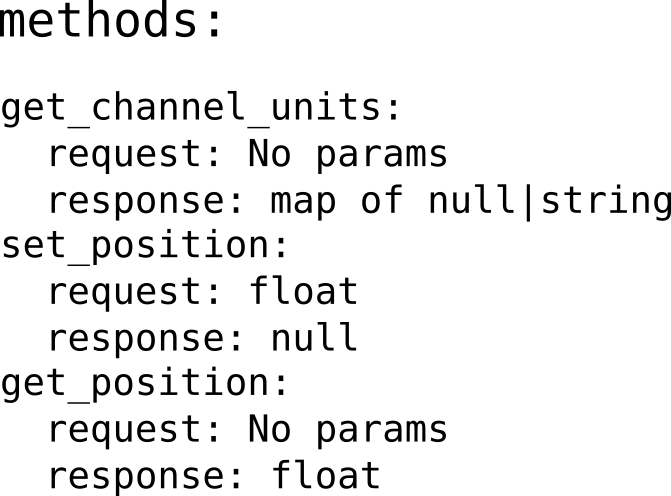
\includegraphics[width=\columnwidth]{./figures/methods.png}
  \caption{  \label{fig:methods} A figure caption. The figure captions are automatically numbered.}
\end{figure}

Once connected, the client will receive an exhaustive description of what capabilities that particular hardware interface supports.
Among this description is a machine-readable summary of what the signature of each remote procedure is.
Figure \ref{fig:methods} summarizes what this might look like.
Here we see three remote procedures, each with a described set of arguments ``request'' and a described response.
As the figure shows, these signatures are typed.
This is only a small piece of the information a client receives.

While Avro RPC itself is agnostic to transport layer, yaq specifies TCP sockets as the transport layer.
TCP socket libraries are ubiquitous, allowing for clients (or daemons) to be implemented in a variety of languages if required.
The use of TCP also works across standard networks, allowing for simple multi-machine instruments.

Apache Avro RPC \cite{AvroSpecification} is used to structure the yaq protcol.
Avro RPC is a Remote Procedure Call framework which allows interprocess communication between a client application and a daemon \(the server\) which has direct hardware access.
Avro provides an agreed upon standard for efficient serialization of data and method calls from a remote \(client\) process.
The protocols defined by Avro are extensible, allowing daemons to define their own data types and declare additional messages that can be processed by the daemon.
Each daemon provides an Avro Protocol file \(avpr\) which provides a complete list of the types and allowed messages.
yaq uses ``stateful'' Avro RPC to allow multiple requests without requiring additional handshaking.

\subsection{Traits}

\begin{figure}
  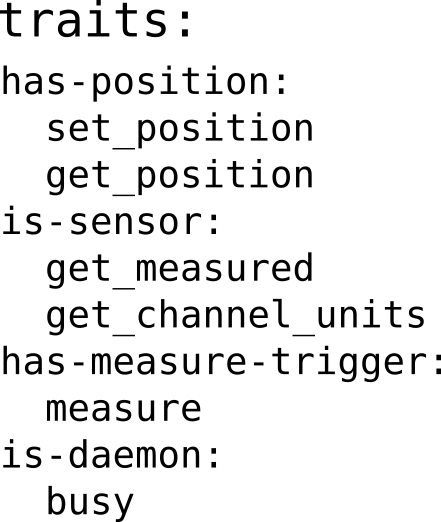
\includegraphics[width=\columnwidth]{./figures/traits.png}
  \caption{  \label{fig:traits} A figure caption. The figure captions are automatically numbered.}
\end{figure}

Each component of a scientific instrument may have many parameters.
Similar components typically have similar parameters, but there may be incidental differences between each implementation.
For example, consider two different monochromators.
The driver for monochromator A may expose the function "set wavelength", while the driver for monochromator B exposes "set angle".
Any experimentalist wishing to switch from monochromator A to B must first go through their entire codebase to fix all of the small differences in the driver implementation.
yaq is designed using an (optional) compositional system that helps enforce consistency between different kinds of hardware.
We call this system ``traits''.

The most basic feature of each trait is a collection of well-defined method signatures, as illustrated by Figure \ref{fig:traits}.
Here, ``has-position'' is a trait and ``set\_position'' and ``get\_position'' are two method signatures defined by that trait.
For brevity we only show method names here, but in reality each method signature is fully described as discussed in the previous section.
Any protocol that wants to implement the ``has-position'' trait must then support those two method signatures.
Importantly, protocols can also implement arbitrary additional methods that are not defined by any trait.

The trait system was introduced in pursuit of our primary goal of easing the client development process.
Clients can trust that protocols that implement a given trait will behave in similar ways.
In Section \ref{sec:clients} we will show how this system makes it easy to write generic clients for a given experiment.
Each trait is carefully defined through prose and examples by an enhancement proposal system that helps the community to gain consensus and serves as living documentation.
These enhancement proposals can be found on the yaq website.

\subsection{Daemons}

\begin{figure}
  \label{fig:daemons}
  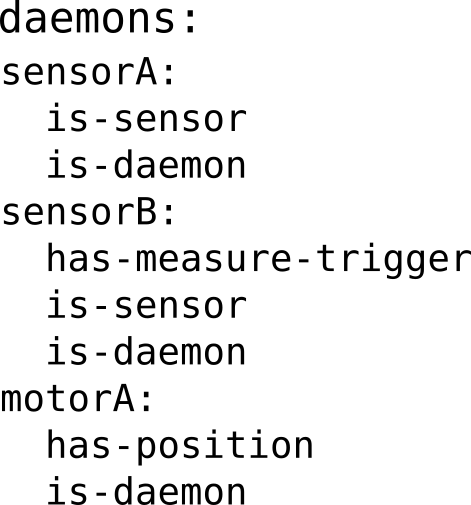
\includegraphics[width=\columnwidth]{./figures/daemons.png}
  \caption{ A figure caption. The figure captions are automatically numbered.}
\end{figure}

In yaq, each component of an instrument is supported by a tiny lightweight process that runs in the background of your computer: a daemon.
Using yaq, a typical instrument has several daemons each supporting a particular component.
As illustrated in Figure \ref{fig:daemons}, each of these daemons has a single protocol which is typically composed of multiple traits as well as unique methods.

Paragraph to describe that methods return quickly and existence of busy.

In yaq, each component of an instrument can be developed and distributed separately.
For example, two very different instruments might happen to use the same temperature sensor.
Because the temperature sensor daemon is its own independent program, both instruments can benefit from the same daemon.
As yaq grows, the "ecosystem" of existing daemons means that future instruments become easier and easier to develop.

There are currently 62 daemons in the yaq project supporting at least 40 kinds of hardware.
Because yaq is protocol based, anyone can design and publish new daemons extending our hardware support.
A living list of all daemons and supported hardware can be found on the yaq website.

\subsection{Clients} \label{sec:clients}

\begin{figure}
  \label{fig:acquisition}
  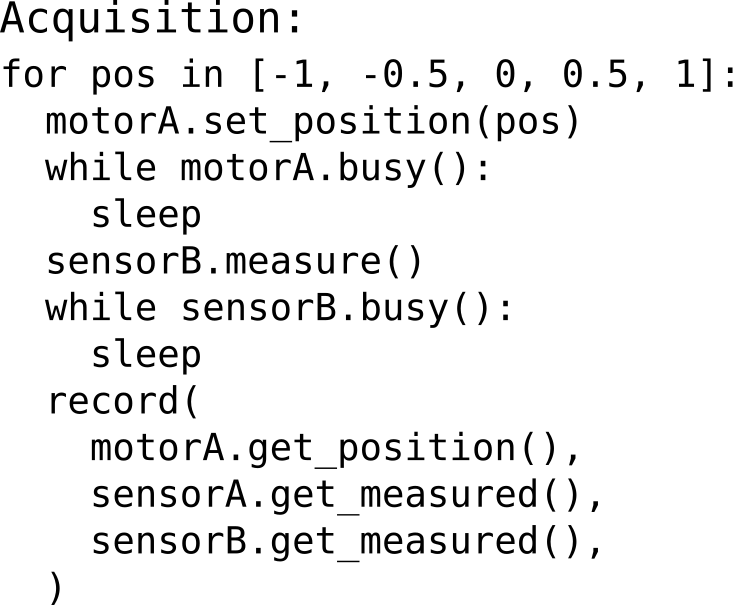
\includegraphics[width=\columnwidth]{./figures/acquisition.png}
  \caption{ A figure caption. The figure captions are automatically numbered.}
\end{figure}

yaq's RPC design invites the creation of multiple client libraries specialized for specific purposes.
Again, daemons can communicate simultaniously with multiple clients.
For a yaq instrument it is normal to have multiple clients running simultaniously, each focused on a particular purpose.
This modularity speeds development and increases overall flexibility of the system.

Figure \ref{fig:acquisition} illustrates using pseudocode what a very basic experimental acquisition might look like using yaq.
Here we have access to the protocols described in Figure \ref{fig:daemons}.
In the outermost for loop the variable ``pos'' is set to a series of different positions.
Each loop iteration involves setting a motor, launching a sensor measurement, then recording all independent and dependent variables.
Because all of these methods are trait-defined, this simple acquisition loop will run as-is for an arbitrary set of motors and sensors.
While this example is simplified, in practice we have found writing simple scripts to drive experiments to be a very productive approach.

yaqc [CITE] is a very basic Python client for yaq.
yaqc is totally generic and aims to support any conceivable yaq RPC.
This library is easy to use directly in Python scripts or within the REPL, but it's also very useful as a dependency when building more specialized Python clients.

yaqc-qtpy [CITE] is a specialty Qt-based [CITE] GUI client.
yaqc-qtpy provides a special QClient object which uses Qt threading primatives to provide performant and safe access to yaq from a Qt environment.
In addition, yaqc-qtpy provides an entry point which automatically builds a GUI from arbitrary protocols using traits.
This is an invaluable tool which provides a ``free'' graphical user interface to any daemon.

Bluesky is an extensive open source control layer developed collaboratively across several user facilities \cite{AllanDanielB2019a}.

Bridging to larger open source control layers.
PyMoDaq \cite{WeberSebastien2021a}

\section{Case Studies}

yaq's simplicity and extensible nature has allowed us to use it in a broad variety of instrumentation designs.
We highlight a few such designs here.

The Landis Group at UW-Madison is currently working on a new type of flow reactor: the Wisconsin Quench Kinetics Reactor (WiQK).
This reactor incorporates several computer-controlled valves and syringe pumps as well as various sensors.
The WiQK is rapidly evolving as researchers continue to test and refine their design.
Only a few researchers are actively using the reactor during this prototyping stage.
The Landis Group has written very basic Python scripts utilizing yaqc to orchestrate hardware for their reactor.
These lightweight scripts can be extensively refactored as the hardware and orchestration strategy changes dramatically during WiQK development.
This approach ensures that the Landis Group is not limited by their ability to orchestrate hardware as they refine their reactor design.

The Stahl Group at UW-Madison created a custom reactor which monitors gasses being produced or consumed in the reaction head-space.  \cite{SalazarChaseA2021a}
This reactor incorporates a collection of sensitive pressure transducers and a single heating process value under computer control.
yaq daemons are used to interface with each sensor and the heater controller.
We were able to create a lightweight Qt-based GUI which offers an easy user experience to researchers.
By separating hardware interface code from GUI code, each piece of the system became easier to produce and maintain.
Taken together, these components have been a solid software experience for many users over several years.

The Wright Group at UW-Madison needs to orchestrate a large variety of hardware in multidimensional scans for their complex spectroscopy experiments \cite{MukamelShaul2000a, WrightJohnCurtis2011a}.
This need for exquisite hardware control has resulted in several prior attempts at ``home-built'' orchestration software \cite{CarlsonRogerJohn1988a, MeyerKentAlbert2004b, KainSchuyler2017a, ThompsonBlaiseJonathan2018a}.
Now, using yaq, the Wright Group has been able to move to Bluesky rather than inventing their own sophisticated control software ``from scratch''.
Moving forward, the Wright Group hopes to spend less energy developing control software and more energy developing creative spectroscopy experiments.

yaq is also being used in several smaller ways throughout UW-Madison Chemistry.
Excitingly, all of these research groups are able easily benefit from each-other's daemon developments.
This level of collaboration is new to us in the orchestration software space.

\section{Conclusion}

TODO

\begin{acknowledgments}
  TODO
\end{acknowledgments}

\section*{Data Availability Statement}

Data sharing is not applicable to this article as no new data were created or analyzed in this study.

\section*{References}

\nocite{*}
\bibliography{references}

\end{document}
